%\VignetteIndexEntry{The ftsa Package}
%\VignetteDepends{ftsa, rainbow, forecast}
%\VignetteKeywords{Functional time series, Functional time series modeling, Functional time series forecasting}
%\VignettePackage{ftsa}

\documentclass[nojss]{jss}

\usepackage{amsmath,amsfonts,bbm,enumitem,microtype,alltt,verbatim,subfig,bm,animate,tikz}
\usepackage[utf8]{inputenc} 
\usepackage[figuresright]{rotating}

\newcommand{\field}[1]{\mathbb{#1}}
\newcommand{\R}{$\field{R}$}
\usetikzlibrary[decorations.shapes]
\usetikzlibrary[petri]
  
%% Change the default page sizes.
  
\setlength{\topmargin}{-0.25in}
\setlength{\textheight}{8.5in}
\setlength{\oddsidemargin}{.0in}
\setlength{\evensidemargin}{.0in}
\setlength{\textwidth}{6.5in}
\setlength{\footskip}{.5in}
  
\newenvironment{smallexample}{\begin{alltt}\small}{\end{alltt}}
\newenvironment{smallverbatim}{\small\verbatim}{\endverbatim}
\graphicspath{{plots/}}
\def\eqd{\stackrel{\mbox{$\scriptstyle  d$}}{=}}

%% need no \usepackage{Sweave.sty}
  
\author{\hspace{-.2in} Piotr Kokoszka, \hspace{0.9in} Han Lin Shang\\Colorado State University, \hspace{.2in} Australian National University} 
  
\title{Stationarity Tests and A New Prediction Method for Functional Time Series}
  
\Plainauthor{Piotr Kokoszka and Han Lin Shang}
  
\Plaintitle{Stationarity Tests and A New Prediction Method for Functional Time Series}
  
\Abstract{
\pkg{ftsa} 4.7 enhances the previous versions by adding tests for stationarity of functional time series and another method for their prediction. A new data set of particulate pollution curves has been added.
}
  
  
\Address{Piotr Kokoszka \\
    Colorado State University \\ 
  Department of Statistics \\
  Fort Collins, CO 80523, USA \\
  E-mail: \email{Piotr.Kokoszka@colostate.edu}\\\\
  Han Lin Shang\\
    Australian National University \\
    Research School of Finance, Actuarial Studies and Statistics \\
    Canberra, ACT 2601, Australia\\
  E-mail: \email{hanlin.shang@anu.edu.au}}

  \Keywords{stationary test, functional time series forecasting, VARMA}
  
  \Plainkeywords{functional data analysis, functional time series}
  
\begin{document}
  

\section{Testing stationarity of functional time series}

A functional time series is a sequence of curves $X_1(t), X_2(t), \ldots, X_N(t)$. Each curve is defined on the same grid of points in an  interval $[T_1, T_2]$. We use $N$ to denote the size of the sample of functions because $t$ is used as the argument of the functions, i.e. a point in the interval $[T_1, T_2]$. In Functional Data Analysis, each function $X_i$ is viewed as an element of a function space, the most general of such spaces is the space of square integrable functions, denoted $L^2 = L^2([T_1, T_2])$ \citep[see e.g.,][Chapter 2]{HKbook}. Just like for scalar and vector time series, many procedures developed for functional time series require that these series be stationary. Function \code{T\_stationary} implements two tests of stationarity developed by \cite{HKR14}. The null hypothesis of these tests is that the series is stationary, in the  strict sense, i.e. that for any $h$ and any $n$ 
\begin{equation}
(X_{1+h}, X_{2+h}, \ldots, X_{n+h}) \eqd (X_{1}, X_{2}, \ldots, X_{n}),
\end{equation}
where the equality in distribution refers to the equality of distributions in the product space $L^2 \times L^2 \times \ldots \times  L^2$ ($n$ times). The alternative hypothesis is that the sequence of functions $X_i$ is not stationary in the above sense. For example, it can contain change points, trends, or random walk components. We emphasize, that each function $t \mapsto X_i(t)$ is typically a realization of a continuous time nonstationary process observed at some discrete points $t_j$. The stationarity refers to the sequence of functions $X_1, X_2, \ldots, X_N$. This point is illustrated in Figure~\ref{f:cidr}. The top panel shows price curves on five consecutive days. Each of these curves can be denoted $X_i$, and only $N=5$ curves are shown. In typical applications,  $N$ is much larger, from several dozen to several thousand. The sequence of price curves is in general not stationary. Even for the five displayed curves an upward trend is seen, such a trending or random walk behavior is much more pronounced for longer series. The Bottom panel of Figure~\ref{f:cidr} shows the same curves, but suitably normalized. Even though each curve is a realization of a nonstationary stochastic process, such normalized curves, known as cumulative intraday return curves \citep[see][and references therein]{kokoszka:miao:zhang:2015}, form a stationary functional time series. 

\begin{figure}[!hbtp]
\centering
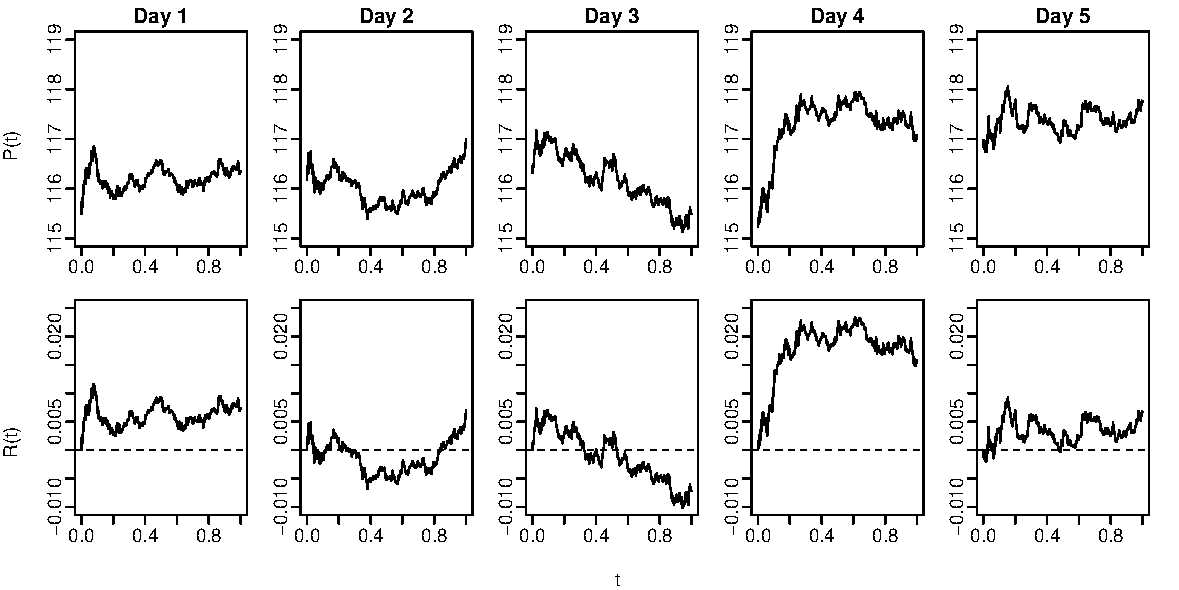
\includegraphics[width=\textwidth]{ibm}
\caption{Top: IBM price curves on five consecutive trading days. Bottom: Cumulative intraday returns on these prices.}\label{f:cidr}
\end{figure}

We illustrate the application of the tests using the functional time series \code{pm\_10\_GR\_sqrt} which has been added to \pkg{ftsa} 4.7 \citep{ftsa}. The data set \code{pm\_10\_GR} contains half--hourly measurements of the concentration of particulate matter less than 10um (pm10) in Graz, Austria from October 1, 2010 to March 31, 2011. This is a functional time series with $N=182$ daily curves. To stabilize variability of these functions, square root of each half--hourly observation is computed; the functional time series so transformed is  available as \code{pm\_10\_GR\_sqrt}. The call 
\begin{Verbatim}
require(ftsa)
T_stationary(pm_10_GR_sqrt$y)
\end{Verbatim} 
produces the following output
\begin{small}
\begin{Verbatim} 
Monte Carlo test of stationarity of a functional time series
null hypothesis: the series is stationary
p-value = 0.082
N (number of functions) = 182
number of MC replications = 1000
\end{Verbatim}
\end{small}
The p--value of 8.2\% indicates that the series can be treated as stationary. Since the p-value is less than 10\%, using a larger sample size might reveal some nonstationarity due to seasonal effects. The null distribution of this test does not have a closed form; it must be approximated by a Monte Carlo distribution. The last line indicates that one thousand replications were used, the default value. The call 
\begin{Verbatim} 
T_stationary(pm_10_GR_sqrt$y, J = 100, MC_rep = 5000, h = 20, pivotal = TRUE)
\end{Verbatim} 
produces the output 
\begin{small}
\begin{Verbatim} 
Pivotal test of stationarity for a functional time series
null hypothesis: the series is stationary
p-value = 0.1188
N (number of functions) = 182
number of MC replications = 5000
\end{Verbatim}
\end{small}
The main difference relative to the previous call is that the argument \code{pivotal = TRUE} indicating that a different tests statistic is used,  which has a pivotal asymptotic distribution. Nevertheless, the distribution of the test statistic is still approximated by a Monte Carlo distribution to ensure a more accurate empirical size. If \code{pivotal = FALSE}, the statistic $T_N$ defined in Section 2.1 of \cite{HKR14} is used; if \code{pivotal = TRUE}, their statistic $T_N^0(d)$ defined in Section 2.2 is used. The argument \code{J} is the truncation level used to approximate the limit distribution defined by an infinite series, only the first $J$ terms of this series are used. The distribution so truncated is used in Monte Carlo replications. The argument $h$ is the kernel bandwidth. Both are defined in Section 4.1 of \cite{HKR14}. The help file of the function \code{T\_stationary} explains other tuning parameters  used in that paper, which are provided  as arguments.  

\section{Forecasting functional time series}

The package \pkg{ftsa} 4.7 implements a new method of predicting functional time series proposed by \cite{ANH15}. The main difference between the new forecasting method implemented in \code{farforecast} and the existing method implemented in \code{forecast.ftsm} is as follows. In both methods, the functions $X_i$ are represented as
\begin{equation}
X_i(t) \approx  \mu(t) + \sum_{j=1}^J \xi_{ij} \hat v_j(t), 
\end{equation} 
where the $\hat v_j$ are the estimated functional principal components, EFPC, \citep[see e.g.,][Chapter 3]{HKbook}. The function \code{forecast.ftsm} treats each series $\xi_{1j}, \xi_{2j}, \xi_{3j}, \ldots, \xi_{Nj}$ as a univariate time series and computes the predictions of its future values using the automatic autoregressive integrated moving average algorithm of \cite{HK08}. These predictions are used to construct the predicted curves using the EFPC decomposition above. The function \code{farforecast} treats the scores as a $J$-dimensional  time series $[\xi_{i1}, \xi_{i2}, \ldots \xi_{iJ}], \ i=1,2,3, \ldots, N$, and applies a multivariate prediction algorithm assuming that this series is a stationary vector autoregression. Before using \code{farforecast} it is therefore advisable to transform the original functional time series to a stationary series and verify stationarity using the function \code{T\_stationary}. Other arguments of the function \code{farforecast} are analogous to the arguments of \code{forecast.ftsm}, and are explained in the help file. 

In Figure~\ref{f:pm10}, we compare the differences between multivariate and univariate time-series forecasting algorithms for predicting one-day-ahead and 30-days-ahead pm10 pollution curves. The following code produces Figure~\ref{f:pm10}. 
\begin{Verbatim}
# Multivariate time-series prediction algorithm
require(ftsa); require(vars)
h30_forecast_sqrt_pm10 = farforecast(ftsm(pm_10_GR_sqrt), h = 30, PI = FALSE)
plot(h30_forecast_sqrt_pm10, ylim = c(5.2,7.5), 
     xlab = "Half hourly intraday time interval",
     ylab = "Forecasts", lwd = 2)
h1_forecast_sqrt_pm10 = farforecast(ftsm(pm_10_GR_sqrt), h = 1)
lines(h1_forecast_sqrt_pm10, lwd = 3, lty = 3)

# Univariate time-series prediction algorithm
h30_forecast_sqrt_pm10_ftsm = forecast(ftsm(pm_10_GR_sqrt), h = 30, method = "arima")
plot(h30_forecast_sqrt_pm10_ftsm, ylim = c(5.2,7.5), lwd = 2)
h1_forecast_sqrt_pm10_ftsm = forecast(ftsm(pm_10_GR_sqrt), h = 1, method = "arima")
lines(h1_forecast_sqrt_pm10_ftsm$mean, lwd = 3, lty = 3)
\end{Verbatim}

\begin{figure}[!htbp]
\centering
\subfloat[Multivariate time-series forecasting algorithm]
{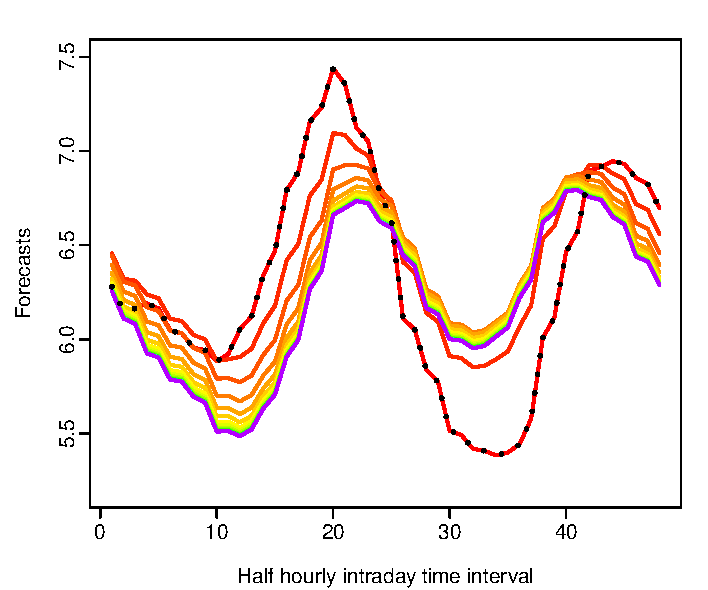
\includegraphics[width=8cm]{pm10}}\quad
\subfloat[Univariate time-series forecasting algorithm]
{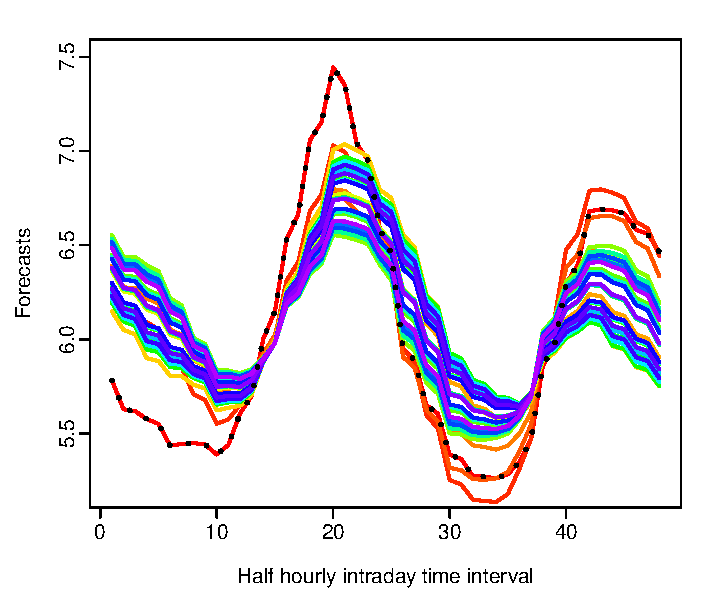
\includegraphics[width=8cm]{pm10_ftsm}}
\caption{Predicted 30--days--ahead pm10 pollution curves; one--day--ahead prediction highlighted with black dots.}\label{f:pm10}
\end{figure}

\section{Conclusion}\label{sec:4}

This article describes a method in the \pkg{ftsa} package for testing the stationarity of a functional time series. For a stationary functional time series, a new prediction method is introduced by forecasting principal component scores via a multivariate time-series forecasting method. Both procedures are illustrated by an application to the concentration of particulate matter data set. We used the test to verify its stationarity, and produced one-step-ahead and 30-steps-ahead forecasts via the new prediction method. To sum up, these two additional methods should be considered when the interest lies in forecasting future realizations of a time series of functions. The test should be used before applying any inferential tools that assume stationarity.



\bibliography{KokoszkaShang}


\end{document}
